Тригонометрические функции представляют собой элементарные функции, аргументом которых является угол. С помощью тригонометрических функций описываются соотношения между сторонами и острыми углами в прямоугольном треугольнике. 

Для построения функций - необходимо вспомнить единичную окружность на которой мы изображали углы и откладывали косинусы и синусы (другое занятие).

\begin{itemize}
    \item Функция синуса $y = \sin{x}$
    
    \begin{figure}[h!]
	\centering
	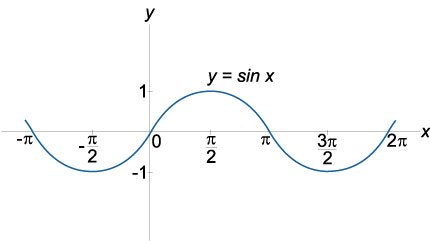
\includegraphics[width=0.5\textwidth]{img/sin.jpg}
    \end{figure}
    
    \item Функция косинуса $y = \cos{x}$
    
    \begin{figure}[h!]
	\centering
	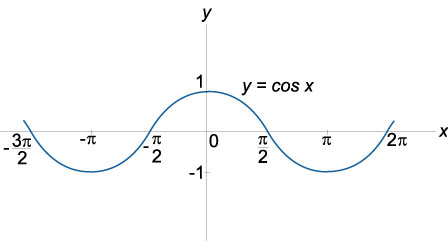
\includegraphics[width=0.5\textwidth]{img/cos.jpg}
    \end{figure}
    
    \item функция тангенса $y = \tg{x}$
    
    \begin{figure}[h!]
	\centering
	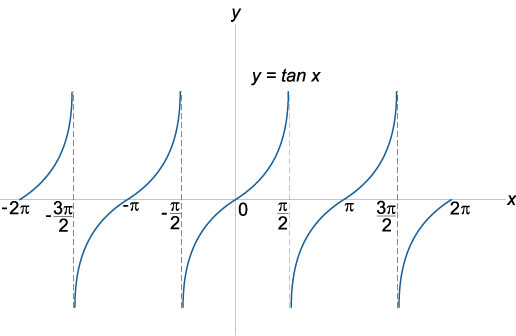
\includegraphics[width=0.5\textwidth]{img/tg.jpg}
    \end{figure}
    
    \item Функция котангенса $y = \ctg{x}$
    
\end{itemize}

\begin{figure}[h!]
\centering
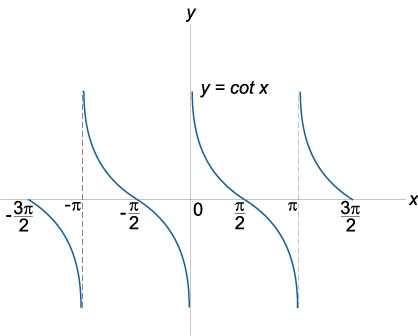
\includegraphics[width=0.5\textwidth]{img/ctg.jpg}
\end{figure}
    
\newpage
Все преобразования, которые мы разбирали здесь также актуальны:

    \begin{figure}[h!]
	\centering
	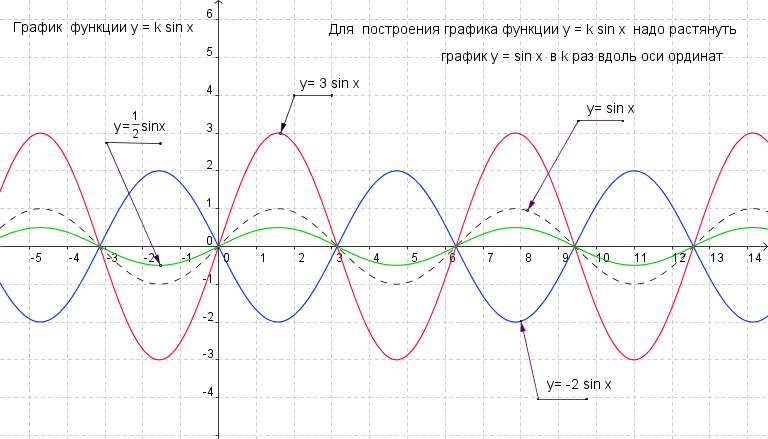
\includegraphics[width=1\textwidth]{img/pr_sin.png}
    \end{figure}